%%%%%%%%%%%%%%%%%%%%%%%%%%%%%%%%%%%%%%%%%%%%%%%%%%%%%%%%%%%%%%%%%%%%%%
%%                     Association
%%%%%%%%%%%%%%%%%%%%%%%%%%%%%%%%%%%%%%%%%%%%%%%%%%%%%%%%%%%%%%%%%%%%%%
%\color{blue}
\subsection{Glyph: \glyph{Association}}\label{sec:association}

The association between two EPNs represents the non-covalent binding of the biological objects represented by those EPNs into a larger complex.

\begin{glyphDescription}
 \item[SBO]\mbox{}\\ SBO:0000177 ! binding.
 \item[origin]\mbox{}\\ More than one \glyph{consumption} arcss (section \ref{sec:consumption}).
 \item[target]\mbox{}\\  One \glyph{production} arc (section \ref{sec:production}).
 \item[node]\mbox{}\\ An \glyph{association} between several entities is represented by a filled disc.
 \end{glyphDescription}

\begin{figure}[H]
  \centering
  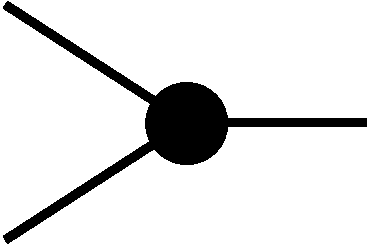
\includegraphics[scale = 0.5]{images/association}
  \caption{The \PD glyph for \glyph{association}.}
  \label{fig:association}
\end{figure}

The following example illustrates the association of two cyclin and CDC2 kinase into the Maturation Promoting Factor in ST.

\begin{center}
\scalebox{0.3}{\includegraphics{examples/association-MPF}}
\end{center}

The following example illustrates the association of a pentameric macromolecule (a nicotinic acetylcholine receptor) with a simple chemical (the local anesthetic chlorpromazin) in an unamed complex, in an ST diagram. 

\begin{center}
\scalebox{0.3}{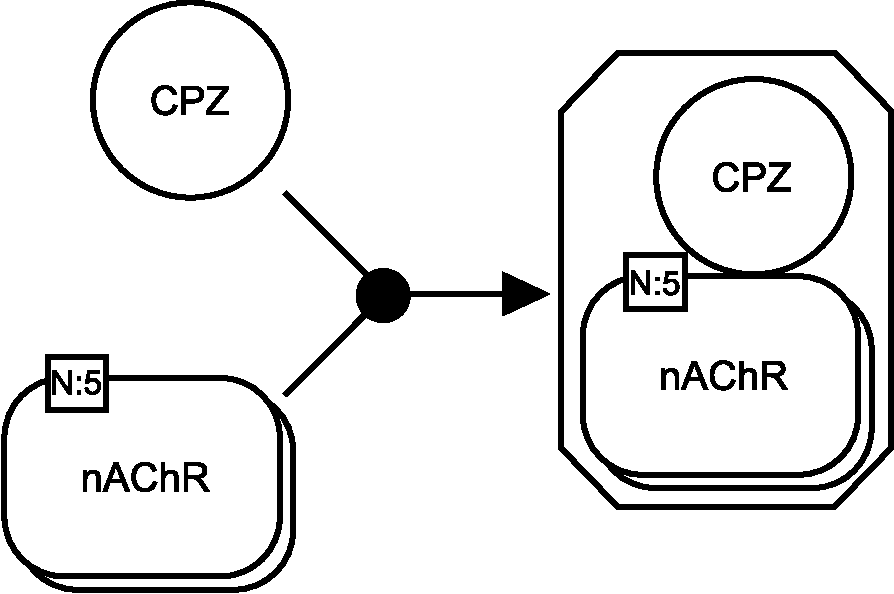
\includegraphics{examples/association-unamed}}
\end{center}

An association does not obligatory results in the formation of a \glyph{complex}, but can also produce a \glyph{multimer}. See the formation of the hemoglobin below.

\begin{center}
\scalebox{0.3}{\includegraphics{examples/association-multimerisation}}
\end{center}
\normalcolor

